%+++++++++++++++++++++++++++++++++++++++++++++++++++++++++++++++
% SUMMARY    : Norms, Inner Product, and Projection
%            : University of Southern Maine 
%            : @james.quinlan
%	     : James Tedder - Lecture 2
%+++++++++++++++++++++++++++++++++++++++++++++++++++++++++++++++

\section*{Objectives}
\begin{outline}
    \1 Norms
    \1 Inner Product
    \1 Projection
\end{outline}

\rule[0.0051in]{\textwidth}{0.00025in}
% ----------------------------------------------------------------
\section{Norms}

A Norm is a function that maps a vector to a real number. It is closely tied to the concepts of absolute value and length. In relation to distance, $||x|| = ||x - 0|| = d(x,0)$. 

The Norm function is $||\cdot|| : V \rightarrow \R^{+}$ such that:

\begin{outline}[enumerate]
	\1 $||x|| \ge 0$    norms are greater than or equal to 0
	\1 $||x|| = 0 \text{ iff } x = 0$    norms are equal to 0 if and only if $x = 0$
	\1 $||Cx|| = |C| \cdot ||x|| \text{ where } C \in \R$
	\1 $||x+y|| \leq ||x|| + ||y||$
\end{outline}

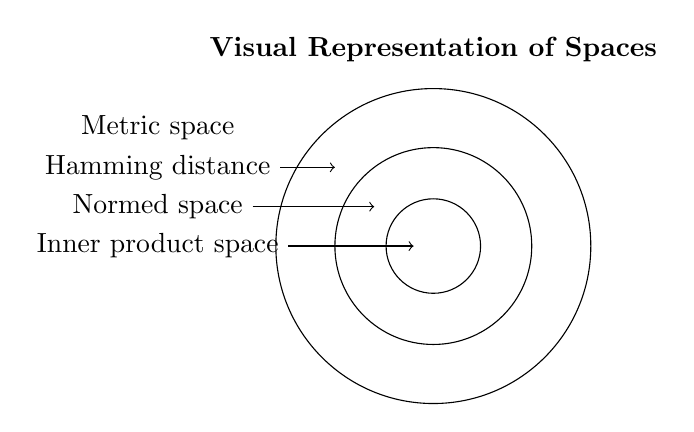
\begin{tikzpicture}[scale=0.5]
    \node[align=center, font=\bfseries] at (0,5) {Visual Representation of Spaces};
    \draw (0,0) circle (4cm); 
    \draw (0,0) circle (2.5cm);
    \draw (0,0) circle (1.2cm);
    \node at (-7,3) (metricLabel) {Metric space};
    \node at (-7, 2) (hammingLabel) {Hamming distance};
    \draw[->] (hammingLabel) -- (-2.5,2);
    \node at (-7,1) (normedLabel) {Normed space};
    \draw[->] (normedLabel) -- (-1.5,1);
    \node at (-7,0) (innerLabel) {Inner product space};
    \draw[->] (innerLabel) -- (-0.5,0);
\end{tikzpicture}

Consider the following example:
% ----------------------------------------------------------------
\[
d_H \left( \mathbf{{x}} = 
\begin{bmatrix}
    1 \\
    0 \\
    1 
\end{bmatrix}, 
\quad
\mathbf{{y}} = 
\begin{bmatrix}
    0 \\
    1 \\
    1 \\
\end{bmatrix} \right) = 2
\]
% ----------------------------------------------------------------

The Hamming Distance must satisfy all properties to be considered a norm function. Consider if $x$ and $y$ were scaled by an arbitrarily chosen constant $3$.
% ----------------------------------------------------------------
\[
d_H \left( \mathbf{{x}} = 
\begin{bmatrix}
    3 \\
    0 \\
    3 
\end{bmatrix}, 
\quad
\mathbf{{y}} = 
\begin{bmatrix}
    0 \\
    3 \\
    3 \\
\end{bmatrix} \right) = 2
\]
% ----------------------------------------------------------------

The Hamming Distance returns the number of elements that differ between two vectors. The result remains the same despite scaling the vectors. Therefore, the Hamming Distance is \textbf{not} a Norm function as it does not meet the third criterion.

\centering
$d_{H}(Cx,Cy) \ne C \cdot d_{H}(x,y)$

\raggedright

There are several types of norms, and we differentiate them by subscripts. The first set of norms are the Minkowski norms or $p$ norms, which are denoted as such:

\centering
1-norm $= ||x||_1$

2-norm $= ||x||_2$

3-norm $= ||x||_3$

p-norm $= ||x||_p$

\raggedright

These norms are calculated differently depending on the subscripts. The equations are shown below. In the first two cases, $p$ is the dimensionality of {\bf x}, and in the third dimension, $n$ is the dimensionality of ${\bf x}$.

\centering
$$||x||_1 = \sum_{i=1}^{p}|x_i|$$

$$||x||_2 = \sqrt{\sum_{x=1}^{p}x_i^2}$$

$$||x||_p = \sqrt{\sum_{i=1}^{n}|x_i|^p}$$

\raggedright

Chebyshev's norm, also referred to as the $\infty$ norm or the max norm, is denoted as $||x||_\infty$. This norm finds the component of the vector that is the farthest from 0 and returns that. The technical definition is as follows.

$$||x||_\infty = max(|x_1|, |x_2|, |x_3|, ... |x_p|)$$

All norms are equivalent but not equal. If $||x||_1$ is larger than $||y||_1$ then $||x||_p$ is larger than $||y||_p$.

\subsection{Sample visualizations of L2 and Chebyshev's Norm}

\begin{tikzpicture}[scale=1.2]
  \tikzset{
    vector/.style={thick, ->, >=stealth},
    level set/.style={thick, dashed, blue},
    point/.style={draw, circle, inner sep=1.5pt, fill=black}
  }

  % Coordinate axes (L2 Norm)
  \draw[thick, ->] (-2,0) -- (2,0) node[right] {$x_1$};
  \draw[thick, ->] (0,-2) -- (0,2) node[above] {$x_2$};

  % L2 norm level sets (circles)

  \draw[level set] (0,0) circle (1.5) node[midway, above right] {};


  % Origin label
  \node[below left] at (0,0) {$0$};
\end{tikzpicture}
\begin{tikzpicture}[scale=1.2]
  \tikzset{
    vector/.style={thick, ->, >=stealth},
    level set/.style={thick, dashed, blue},
    point/.style={draw, circle, inner sep=1.5pt, fill=black}
  }

  % Coordinate axes (Chebyshev Norm)
  \draw[thick, ->] (-2,0) -- (2,0) node[right] {$x_1$};
  \draw[thick, ->] (0,-2) -- (0,2) node[above] {$x_2$};

  % Chebyshev norm level sets (squares)

  \draw[level set] (-1.5,-1.5) rectangle (1.5,1.5) node[midway, fill=white, inner sep=1pt] {};


\end{tikzpicture}


% ----------------------------------------------------------------
\section{Inner Product}

The inner product is $\langle\cdot,\cdot\rangle: V \times V \rightarrow\R$ such that:

\begin{outline}[enumerate]
	\1 $\langle x,x \rangle \geq 0$
	\1 $\langle x,x \rangle = 0 \text{iff} x=0$
	\1 $\langle x,y \rangle = \langle y,x \rangle$
	\1 $\langle \alpha x+ \beta y,z \rangle = \alpha \langle x,z \rangle + \beta \langle y,z \rangle$, $\alpha,\beta \in \R$,
			$x,y,z \in V$
\end{outline}

This is the basis of the neural networks. A few more aspects of the inner product are:

\vspace{0.8em} 

$\langle x,y \rangle = x^T y = \sum_{i=1}^{P}x_i y_i$

\vspace{1em} 

In the diagram below, the vector $x$ contains three input features, and each connection
to the output node is weighted by a corresponding component of $y$. The output results from computing the dot product $\langle x, y \rangle$, and then adding a bias $b$. 
This is the fundamental operation of a single neuron in a neural network.


\begin{center}
	\begin{minipage}[c]{0.35\textwidth}
		\begin{align*}
			x &= \begin{bmatrix} x_1 \\ x_2 \\ x_3 \end{bmatrix}
		\end{align*}
	\end{minipage}
	\hfill
	\begin{minipage}[c]{0.6\textwidth}
		\resizebox{!}{5cm}{
			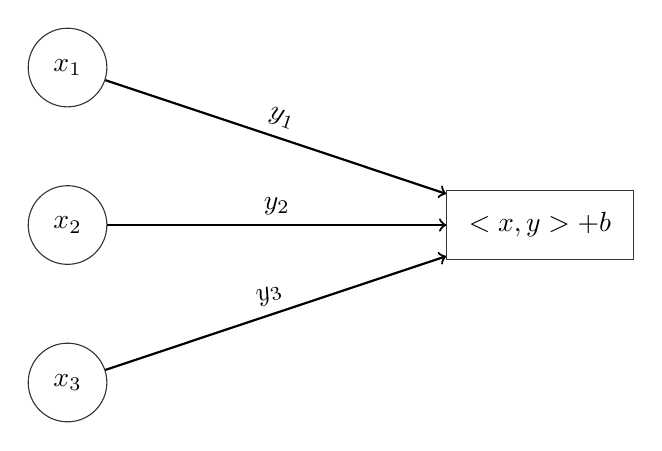
\begin{tikzpicture}
				% Input nodes (features)
				\node[circle, draw=black!80, inner sep=6pt] (x1) at (0,6) {$x_1$};
				\node[circle, draw=black!80, inner sep=6pt] (x2) at (0,4) {$x_2$};
				\node[circle, draw=black!80, inner sep=6pt] (x3) at (0,2) {$x_3$};

				% Output node (prediction)
				\node[rectangle, draw=black!80, inner sep=8pt] (output) at (6,4) {$<x,y> + b$};
		
				% Weights and connections
				\draw[thick, ->] (x1) -- node[midway, above, sloped] {\(y_1\)} (output);
				\draw[thick, ->] (x2) -- node[midway, above, sloped] {\(y_2\)} (output);
				\draw[thick, ->] (x3) -- node[midway, above, sloped] {\(y_3\)} (output);
		
			\end{tikzpicture}
		}
	\end{minipage}
\end{center}

An important special case of the inner product occurs when a vector is dotted 
with itself. This gives us the 2-norm, of the vector:

\vspace{0.8em} 

$||x|| = \sqrt{\langle x,x \rangle}$


% ----------------------------------------------------------------
\section{Projection}

Projection is used in principal component analysis. We started by looking at the problem to show a situation in which projection might be necessary.

$Ax=b$

A is a 2d matrix, b is a known vector, and x is an unknown vector.

$\begin{bmatrix}
1 & 2 & 3\\
4 & 5 & 6\\
7 & 8 & 9
\end{bmatrix}
\begin{pmatrix}
x_1\\
x_2\\
x_3
\end{pmatrix}
=
\begin{pmatrix}
10\\
11\\
12
\end{pmatrix}$

This problem has us trying to find the vector x. 
This problem may have no perfect solution. 
This is the sort of problem where we might use projection to solve it because projection is the best solution we can come up with.

He then showed another problem.

\begin{tikzpicture}
	\draw[thick,->] (0,0) -- (4.5,0) node[anchor=north west] {x axis};
	\draw[thick,->] (0,0) -- (0,4.5) node[anchor=south east] {y axis};
	\draw[thick,->] (0,0) -- (4,1) node[anchor=south east] {a};
	\draw[thick,->] (0,0) -- (2.5,2) node[anchor=south east] {b};
\end{tikzpicture}

The goal was to project $b$ down onto $a$. This is necessary because there is no way to turn $a$ into $b$ through multiplication. Multiplication just stretches vector $a$. We'll need to know a few terms before we can do this.

$p =$ projection which is equivalent to $b_\|$ which is parallel to $a$. It is equivalent to $a$ times some constant as it is just a resizing of $a$ or $b_\| = ca = p$. This is the vector added below.

\begin{tikzpicture}
	\draw[thick,->] (0,0) -- (4.5,0) node[anchor=north west] {x axis};
	\draw[thick,->] (0,0) -- (0,4.5) node[anchor=south east] {y axis};
	\draw[thick,->] (0,0) -- (4,1) node[anchor=south east] {a};
	\draw[thick,->] (0,0) -- (2.5,2) node[anchor=south east] {b};
	\draw[thick,->] (0,0) -- (3,0.75) node[anchor=north east] {$b_\|$};
\end{tikzpicture}

$b_\perp$ is perpendicular to $a$. It is also known as the residual and equals $b$ minus $a$ times some constant $c$, or $b_\perp = b-ca$. This is the vector added below.

\begin{tikzpicture}
	\draw[thick,->] (0,0) -- (4.5,0) node[anchor=north west] {x axis};
	\draw[thick,->] (0,0) -- (0,4.5) node[anchor=south east] {y axis};
	\draw[thick,->] (0,0) -- (4,1) node[anchor=south east] {a};
	\draw[thick,->] (0,0) -- (2.5,2) node[anchor=south east] {b};
	\draw[thick,->] (0,0) -- (3,0.75) node[anchor=north west] {$b_\|$};
	\draw[thick,->] (2.5,2) -- (3,0.75) node[anchor=south east] {$b_\perp$};
\end{tikzpicture}

It is also important to note that $b = b_\| + b_\perp$ and that $\langle b_\| , b_\perp \rangle = 0$ we use all of these definitions and the inner product to solve it.

\begin{align*}
    \langle b_{\parallel}, b_{\perp} \rangle &= 0 \\
    \\
    \langle b_{\parallel}, b_{\perp} \rangle &= \langle ca, b-ca \rangle \\
    &= (ca)^T(b-ca) \\
    &= ca^T (b-ca) \\
    &= ca^Tb-c^2a^Ta \\ 
    ca^Tb-c^2a^Ta &= 0 \\
    c^2a^Ta  &= ca^Tb \\
    ca^Ta  &= a^Tb \\
    c &= \frac{a^Tb}{a^Ta} \\
    &= \frac{\langle a,b\rangle}{\langle a,a\rangle} \\
    ca &= \frac{\langle a,b\rangle}{\langle a,a\rangle} a \\
    P &= ca
\end{align*}

All of this allows you to project $b$ onto $a$.
